% Options for packages loaded elsewhere
\PassOptionsToPackage{unicode}{hyperref}
\PassOptionsToPackage{hyphens}{url}
%
\documentclass[
]{article}
\usepackage{amsmath,amssymb}
\usepackage{lmodern}
\usepackage{iftex}
\ifPDFTeX
  \usepackage[T1]{fontenc}
  \usepackage[utf8]{inputenc}
  \usepackage{textcomp} % provide euro and other symbols
\else % if luatex or xetex
  \usepackage{unicode-math}
  \defaultfontfeatures{Scale=MatchLowercase}
  \defaultfontfeatures[\rmfamily]{Ligatures=TeX,Scale=1}
\fi
% Use upquote if available, for straight quotes in verbatim environments
\IfFileExists{upquote.sty}{\usepackage{upquote}}{}
\IfFileExists{microtype.sty}{% use microtype if available
  \usepackage[]{microtype}
  \UseMicrotypeSet[protrusion]{basicmath} % disable protrusion for tt fonts
}{}
\makeatletter
\@ifundefined{KOMAClassName}{% if non-KOMA class
  \IfFileExists{parskip.sty}{%
    \usepackage{parskip}
  }{% else
    \setlength{\parindent}{0pt}
    \setlength{\parskip}{6pt plus 2pt minus 1pt}}
}{% if KOMA class
  \KOMAoptions{parskip=half}}
\makeatother
\usepackage{xcolor}
\usepackage[margin=1in]{geometry}
\usepackage{color}
\usepackage{fancyvrb}
\newcommand{\VerbBar}{|}
\newcommand{\VERB}{\Verb[commandchars=\\\{\}]}
\DefineVerbatimEnvironment{Highlighting}{Verbatim}{commandchars=\\\{\}}
% Add ',fontsize=\small' for more characters per line
\usepackage{framed}
\definecolor{shadecolor}{RGB}{248,248,248}
\newenvironment{Shaded}{\begin{snugshade}}{\end{snugshade}}
\newcommand{\AlertTok}[1]{\textcolor[rgb]{0.94,0.16,0.16}{#1}}
\newcommand{\AnnotationTok}[1]{\textcolor[rgb]{0.56,0.35,0.01}{\textbf{\textit{#1}}}}
\newcommand{\AttributeTok}[1]{\textcolor[rgb]{0.77,0.63,0.00}{#1}}
\newcommand{\BaseNTok}[1]{\textcolor[rgb]{0.00,0.00,0.81}{#1}}
\newcommand{\BuiltInTok}[1]{#1}
\newcommand{\CharTok}[1]{\textcolor[rgb]{0.31,0.60,0.02}{#1}}
\newcommand{\CommentTok}[1]{\textcolor[rgb]{0.56,0.35,0.01}{\textit{#1}}}
\newcommand{\CommentVarTok}[1]{\textcolor[rgb]{0.56,0.35,0.01}{\textbf{\textit{#1}}}}
\newcommand{\ConstantTok}[1]{\textcolor[rgb]{0.00,0.00,0.00}{#1}}
\newcommand{\ControlFlowTok}[1]{\textcolor[rgb]{0.13,0.29,0.53}{\textbf{#1}}}
\newcommand{\DataTypeTok}[1]{\textcolor[rgb]{0.13,0.29,0.53}{#1}}
\newcommand{\DecValTok}[1]{\textcolor[rgb]{0.00,0.00,0.81}{#1}}
\newcommand{\DocumentationTok}[1]{\textcolor[rgb]{0.56,0.35,0.01}{\textbf{\textit{#1}}}}
\newcommand{\ErrorTok}[1]{\textcolor[rgb]{0.64,0.00,0.00}{\textbf{#1}}}
\newcommand{\ExtensionTok}[1]{#1}
\newcommand{\FloatTok}[1]{\textcolor[rgb]{0.00,0.00,0.81}{#1}}
\newcommand{\FunctionTok}[1]{\textcolor[rgb]{0.00,0.00,0.00}{#1}}
\newcommand{\ImportTok}[1]{#1}
\newcommand{\InformationTok}[1]{\textcolor[rgb]{0.56,0.35,0.01}{\textbf{\textit{#1}}}}
\newcommand{\KeywordTok}[1]{\textcolor[rgb]{0.13,0.29,0.53}{\textbf{#1}}}
\newcommand{\NormalTok}[1]{#1}
\newcommand{\OperatorTok}[1]{\textcolor[rgb]{0.81,0.36,0.00}{\textbf{#1}}}
\newcommand{\OtherTok}[1]{\textcolor[rgb]{0.56,0.35,0.01}{#1}}
\newcommand{\PreprocessorTok}[1]{\textcolor[rgb]{0.56,0.35,0.01}{\textit{#1}}}
\newcommand{\RegionMarkerTok}[1]{#1}
\newcommand{\SpecialCharTok}[1]{\textcolor[rgb]{0.00,0.00,0.00}{#1}}
\newcommand{\SpecialStringTok}[1]{\textcolor[rgb]{0.31,0.60,0.02}{#1}}
\newcommand{\StringTok}[1]{\textcolor[rgb]{0.31,0.60,0.02}{#1}}
\newcommand{\VariableTok}[1]{\textcolor[rgb]{0.00,0.00,0.00}{#1}}
\newcommand{\VerbatimStringTok}[1]{\textcolor[rgb]{0.31,0.60,0.02}{#1}}
\newcommand{\WarningTok}[1]{\textcolor[rgb]{0.56,0.35,0.01}{\textbf{\textit{#1}}}}
\usepackage{longtable,booktabs,array}
\usepackage{calc} % for calculating minipage widths
% Correct order of tables after \paragraph or \subparagraph
\usepackage{etoolbox}
\makeatletter
\patchcmd\longtable{\par}{\if@noskipsec\mbox{}\fi\par}{}{}
\makeatother
% Allow footnotes in longtable head/foot
\IfFileExists{footnotehyper.sty}{\usepackage{footnotehyper}}{\usepackage{footnote}}
\makesavenoteenv{longtable}
\usepackage{graphicx}
\makeatletter
\def\maxwidth{\ifdim\Gin@nat@width>\linewidth\linewidth\else\Gin@nat@width\fi}
\def\maxheight{\ifdim\Gin@nat@height>\textheight\textheight\else\Gin@nat@height\fi}
\makeatother
% Scale images if necessary, so that they will not overflow the page
% margins by default, and it is still possible to overwrite the defaults
% using explicit options in \includegraphics[width, height, ...]{}
\setkeys{Gin}{width=\maxwidth,height=\maxheight,keepaspectratio}
% Set default figure placement to htbp
\makeatletter
\def\fps@figure{htbp}
\makeatother
\setlength{\emergencystretch}{3em} % prevent overfull lines
\providecommand{\tightlist}{%
  \setlength{\itemsep}{0pt}\setlength{\parskip}{0pt}}
\setcounter{secnumdepth}{-\maxdimen} % remove section numbering
\usepackage{titlesec}
\titleformat*{\section}{\normalfont\Large\bfseries\flushleft}
\titleformat*{\subsection}{\normalfont\large\bfseries\flushleft}
\titleformat*{\subsubsection}{\normalfont\normalsize\bfseries\flushleft}
\ifLuaTeX
  \usepackage{selnolig}  % disable illegal ligatures
\fi
\IfFileExists{bookmark.sty}{\usepackage{bookmark}}{\usepackage{hyperref}}
\IfFileExists{xurl.sty}{\usepackage{xurl}}{} % add URL line breaks if available
\urlstyle{same} % disable monospaced font for URLs
\hypersetup{
  pdftitle={Statistical Learning (5454) - Assignment 2},
  pdfauthor={Matthias Hochholzer, Lukas Pirnbacher, Anne Valder},
  hidelinks,
  pdfcreator={LaTeX via pandoc}}

\title{Statistical Learning (5454) - Assignment 2}
\author{Matthias Hochholzer, Lukas Pirnbacher, Anne Valder}
\date{Due: 2024-04-22}

\begin{document}
\maketitle

\hypertarget{exercise-1}{%
\section{Exercise 1}\label{exercise-1}}

After generating the simulated data we fit four models using least
squares, we calculate the AIC values and determine the in-sample error
estimates by drawing suitable test data from the data generating process
using twice the negative log-likelihood as loss function. Plotting the
data we see a clearly non-linear relationship. In line with this we
observe that the most preferable model in terms of AIC value is the
second model. In terms of negative log-likelihood the fourth model
appears to be the best. However, closely followed by model 2. The linear
model (model 1) performs the worst out of all models measured by AIC and
the negative log-likelihood.

\begin{Shaded}
\begin{Highlighting}[]
\CommentTok{\#(a)}
\FunctionTok{set.seed}\NormalTok{(}\DecValTok{1}\NormalTok{)}
\NormalTok{x }\OtherTok{\textless{}{-}} \FunctionTok{rnorm}\NormalTok{(}\DecValTok{100}\NormalTok{)}
\NormalTok{y }\OtherTok{\textless{}{-}}\NormalTok{ x }\SpecialCharTok{{-}} \DecValTok{2}\SpecialCharTok{*}\NormalTok{x}\SpecialCharTok{\^{}}\DecValTok{2} \SpecialCharTok{+} \FunctionTok{rnorm}\NormalTok{(}\DecValTok{100}\NormalTok{)}
\FunctionTok{plot}\NormalTok{(x,y)}
\end{Highlighting}
\end{Shaded}

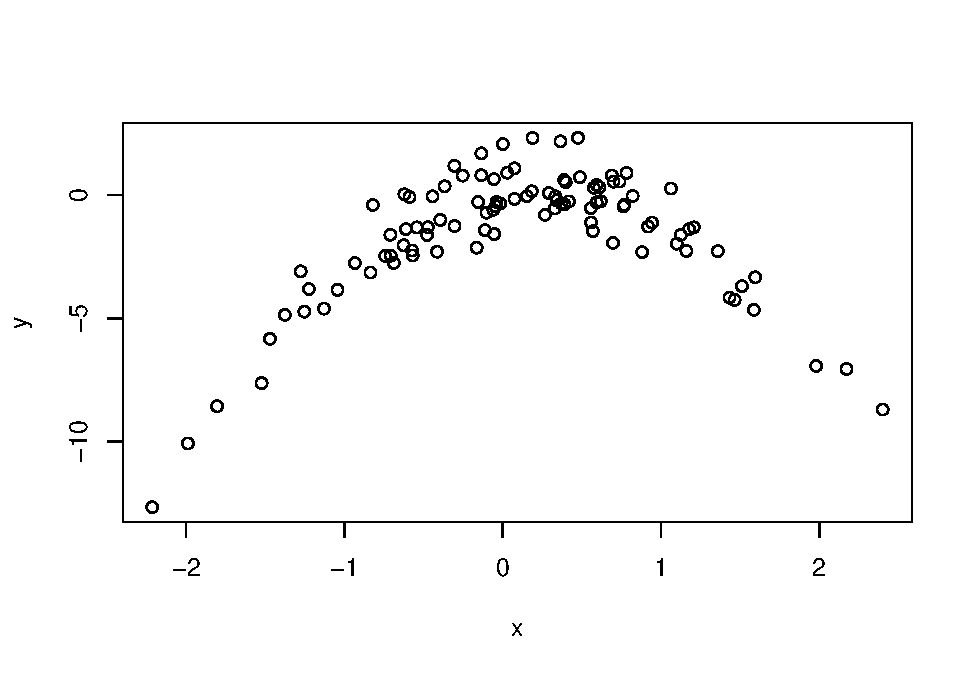
\includegraphics{A2_files/figure-latex/unnamed-chunk-3-1.pdf}

\begin{Shaded}
\begin{Highlighting}[]
\CommentTok{\#(b) model specifications:}
\NormalTok{lm1 }\OtherTok{\textless{}{-}} \FunctionTok{lm}\NormalTok{(y }\SpecialCharTok{\textasciitilde{}}\NormalTok{ x) }\CommentTok{\# alternative: lm1 \textless{}{-} glm(y \textasciitilde{} x, data, family = gaussian()) }
\NormalTok{lm2 }\OtherTok{\textless{}{-}} \FunctionTok{lm}\NormalTok{(y }\SpecialCharTok{\textasciitilde{}}\NormalTok{ x }\SpecialCharTok{+}\FunctionTok{I}\NormalTok{(x}\SpecialCharTok{\^{}}\DecValTok{2}\NormalTok{))}
\NormalTok{lm3 }\OtherTok{\textless{}{-}} \FunctionTok{lm}\NormalTok{(y }\SpecialCharTok{\textasciitilde{}}\NormalTok{ x }\SpecialCharTok{+} \FunctionTok{I}\NormalTok{(x}\SpecialCharTok{\^{}}\DecValTok{2}\NormalTok{) }\SpecialCharTok{+} \FunctionTok{I}\NormalTok{(x}\SpecialCharTok{\^{}}\DecValTok{3}\NormalTok{))}
\NormalTok{lm4 }\OtherTok{\textless{}{-}} \FunctionTok{lm}\NormalTok{(y }\SpecialCharTok{\textasciitilde{}}\NormalTok{ x }\SpecialCharTok{+} \FunctionTok{I}\NormalTok{(x}\SpecialCharTok{\^{}}\DecValTok{2}\NormalTok{) }\SpecialCharTok{+} \FunctionTok{I}\NormalTok{(x}\SpecialCharTok{\^{}}\DecValTok{3}\NormalTok{) }\SpecialCharTok{+} \FunctionTok{I}\NormalTok{(x}\SpecialCharTok{\^{}}\DecValTok{4}\NormalTok{))}
\end{Highlighting}
\end{Shaded}

\begin{verbatim}
## [1] 478.8804 280.1670 282.0886 282.2963
\end{verbatim}

\begin{verbatim}
## [[1]]
## 'log Lik.' 526.7693 (df=3)
## 
## [[2]]
## 'log Lik.' 279.7447 (df=4)
## 
## [[3]]
## 'log Lik.' 522.8529 (df=4)
## 
## [[4]]
## 'log Lik.' 278.7059 (df=6)
\end{verbatim}

\hypertarget{exercise-2}{%
\section{Exercise 2}\label{exercise-2}}

In exercise 2, we perform leave-one-out cross-validation (LOOCV), k-fold
cross-validation (kCV) and empirical bootstrapping based on the mean
squared error loss that result from fitting the four models using least
squares. The simulated data and specifications are the same as in task
1. The results of task (b) across the models are shown in table 1,
incidcated by ``seed1'' in the last column.

\begin{enumerate}
\def\labelenumi{(\alph{enumi})}
\setcounter{enumi}{2}
\tightlist
\item
  Next, we repeat (b) using another random seed (indicated by ``seed2''
  in table 1). For LOOCV we obtain exactly the same results for all four
  models regardless of the different seed. This is because in general
  the randomness lies in the data generation.This consistency is
  expected because LOOCV is deterministic in this context, not relying
  on random sampling. Each observation is used once as a test set while
  the rest are used for training, and this process is repeated for each
  observation in the dataset. Therefore, changing the seed does not
  affect LOOCV results. For kCV we observe slight differences in the
  errors between seed 1 and seed 2 across the models. This variation can
  be attributed to the random partitioning of the data into k folds.
  Each seed leads to a different random split, which can result in
  slight variations in the training and validation sets used in each
  fold, thus affecting the error estimates. Similar to kCV, the
  bootstrap error shows variations between the two seeds. Bootstrap
  resampling involves drawing samples with replacement from the original
  data set to create ``new'' data sets. The randomness introduced by the
  seed affects which observations are selected in each resample, leading
  to slight differences in the bootstrap error estimates between seed 1
  and seed 2.
\end{enumerate}

\begin{longtable}[]{@{}lrrrll@{}}
\caption{Comparison of LOOCV, kCV, and Bootstrap Errors}\tabularnewline
\toprule()
& LOOCV & kCV & Bootstrap & Model & Seed \\
\midrule()
\endfirsthead
\toprule()
& LOOCV & kCV & Bootstrap & Model & Seed \\
\midrule()
\endhead
1 & 7.2882 & 6.1856 & 6.2931 & Model 1 & Seed1 \\
5 & 7.2882 & 6.4165 & 6.2764 & Model 1 & Seed2 \\
2 & 0.9374 & 0.9230 & 0.8702 & Model 2 & Seed1 \\
6 & 0.9374 & 0.9012 & 0.8704 & Model 2 & Seed2 \\
3 & 0.9566 & 0.9316 & 0.8554 & Model 3 & Seed1 \\
7 & 0.9566 & 0.8854 & 0.8557 & Model 3 & Seed2 \\
4 & 0.9539 & 0.9247 & 0.8393 & Model 4 & Seed1 \\
8 & 0.9539 & 0.8962 & 0.8452 & Model 4 & Seed2 \\
\bottomrule()
\end{longtable}

\begin{enumerate}
\def\labelenumi{(\alph{enumi})}
\setcounter{enumi}{3}
\item
  The MSEs in table 1 suggest that according to LOOCV the second model
  is the best. With kCV the third model is the best and for the
  empirical bootstrap error it is the fourth model. Also, we see that
  the empirical bootstrap error decreases further with model complexity,
  reflecting potential overfitting problems of this method. Remembering
  the plotted data in the beginning these results are in line with our
  expectations since higher order regression equations fit much better
  to the data than the linear case.
\item
  Last, we have a look at the statistical significance of the
  coefficient estimates that result from fitting each of the models
  using least squares. The results here align with our previous
  conclusions, as the quadratic term has the lowest p-value.
  \textbackslash begin\{table\}
\end{enumerate}

\centering
\begin{tabular}[t]{l|r|r|r|r}
\hline
  & Estimate & Std. Error & t value & Pr(>|t|)\\
\hline
(Intercept) & -1.625427 & 0.2619366 & -6.205420 & 0.0000000\\
\hline
x & 0.692497 & 0.2909418 & 2.380191 & 0.0192385\\
\hline
\end{tabular}
\centering
\begin{tabular}[t]{l|r|r|r|r}
\hline
  & Estimate & Std. Error & t value & Pr(>|t|)\\
\hline
(Intercept) & 0.056715 & 0.1176555 & 0.482043 & 0.6308613\\
\hline
x & 1.017161 & 0.1079827 & 9.419666 & 0.0000000\\
\hline
I(x\textasciicircum{}2) & -2.118921 & 0.0847657 & -24.997388 & 0.0000000\\
\hline
\end{tabular}
\centering
\begin{tabular}[t]{l|r|r|r|r}
\hline
  & Estimate & Std. Error & t value & Pr(>|t|)\\
\hline
(Intercept) & 0.0615072 & 0.1195037 & 0.5146883 & 0.6079538\\
\hline
x & 0.9752803 & 0.1872815 & 5.2075636 & 0.0000011\\
\hline
I(x\textasciicircum{}2) & -2.1237910 & 0.0870025 & -24.4106856 & 0.0000000\\
\hline
I(x\textasciicircum{}3) & 0.0176386 & 0.0642904 & 0.2743580 & 0.7843990\\
\hline
\end{tabular}
\centering
\begin{tabular}[t]{l|r|r|r|r}
\hline
  & Estimate & Std. Error & t value & Pr(>|t|)\\
\hline
(Intercept) & 0.1567030 & 0.1394619 & 1.1236253 & 0.2640034\\
\hline
x & 1.0308256 & 0.1913365 & 5.3874999 & 0.0000005\\
\hline
I(x\textasciicircum{}2) & -2.4098982 & 0.2348551 & -10.2612148 & 0.0000000\\
\hline
I(x\textasciicircum{}3) & -0.0091329 & 0.0672288 & -0.1358481 & 0.8922288\\
\hline
I(x\textasciicircum{}4) & 0.0697854 & 0.0532401 & 1.3107691 & 0.1930956\\
\hline
\end{tabular}

\textbackslash end\{table\}

\hypertarget{exercise-3}{%
\section{Exercise 3}\label{exercise-3}}

Here we are using the wage data set available as data object
\(\textit{Schooling}\) in package \(\textbf{Ecda}\). First, we omit
observations with missing values and the variable wage76, and mutate
variable mar76 into a binary variable. Next, we fit regularized linear
regression models with lwage76 as dependent variable using only linear
effects for the covariates and varying the \(\alpha\) parameter for the
elastic from 0 to 1 in step sizes of 0.2. We do this using using
cv.glmnet with 10-fold cross-validation considering the MSE for a range
of penalty values of \(\lambda\). The argument foldid ensures that the
same data partitions are used for each model fitting, making the
comparisons fair and consistent. The default plot method for cv.glmnet
objects is used to visualize the cross-validation curves, which show the
mean squared error (MSE) across a range of \(\lambda\) values for each
\(\alpha\). The plot displays the \(\lambda\) values on the log scale
along the bottom x-axis and the corresponding MSE on the y-axis. The
vertical dotted line in each plot indicates the \(\lambda\) value that
gives the minimum MSE. By varying \(\alpha\), we essentially move
between different regularization methods: \(\alpha = 0\) corresponds to
ridge regression (penalty on the square of coefficients),\(\alpha = 1\)
corresponds to lasso regression (penalty on the absolute value of
coefficients). The top x-axis shows these numbers, which correspond to
the model's complexity at different levels of regularization. As lambda
increases, the regularization penalty becomes more severe, leading to
more coefficients being shrunk to zero.The dual x-axes in the plot serve
to simultaneously convey how lambda affects both the model's predictive
accuracy (through the MSE shown on the y-axis) and its complexity (in
terms of the number of predictors used, shown on the bottom x-axis).
Looking at the different plots given each value of \(\alpha\) we observe
with \(\alpha\) closer to 1 more pronounced changes in the number of
non-zero coefficients as lambda changes, reflecting the lasso's variable
selection property. For ridge regression (\(\alpha = 0\) ), the
coefficients are shrunk towards zero but not exactly to zero, so the
model complexity in terms of the non-zero coefficient count may not
reduce as dramatically as with lasso or elastic net.

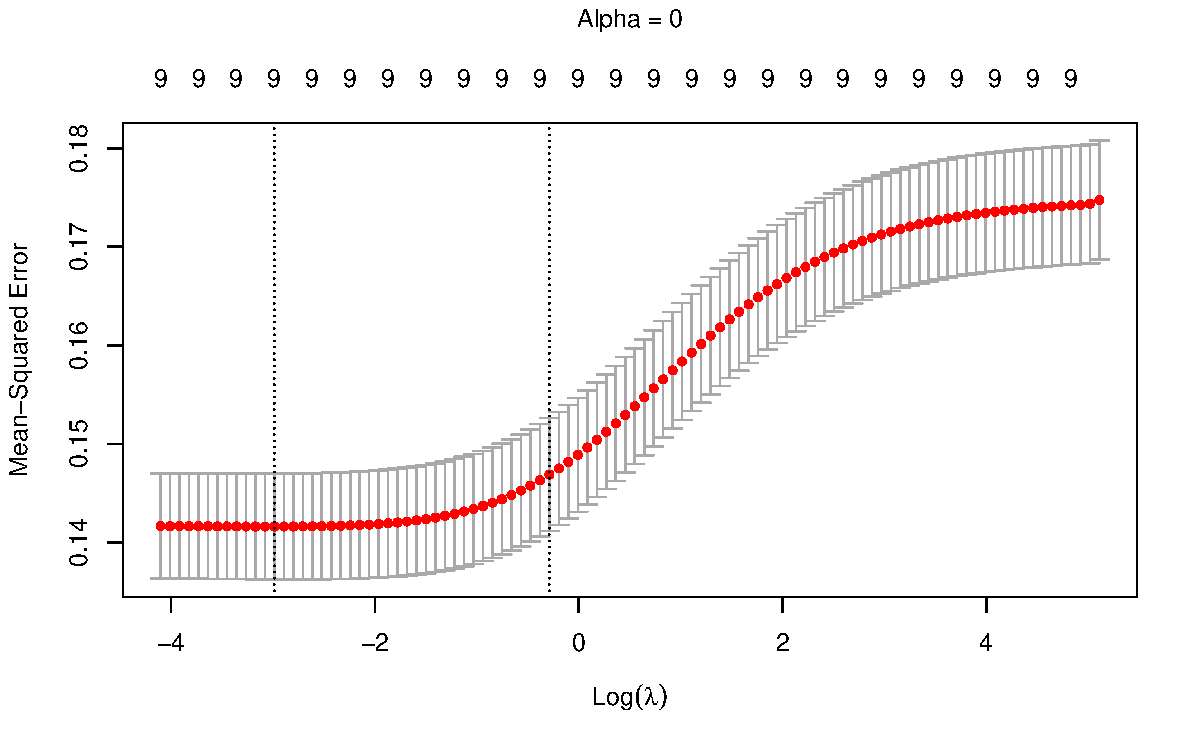
\includegraphics[width=\textwidth]{A2_files/figure-latex/unnamed-chunk-7-1}
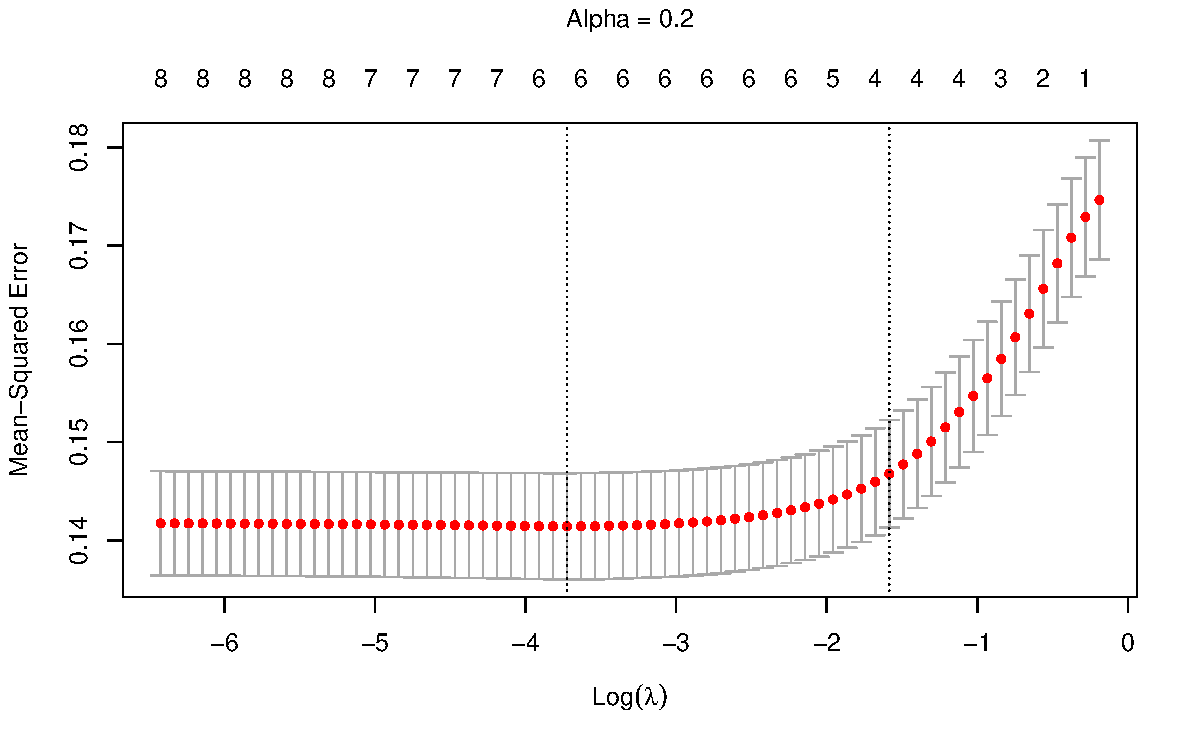
\includegraphics[width=\textwidth]{A2_files/figure-latex/unnamed-chunk-7-2}
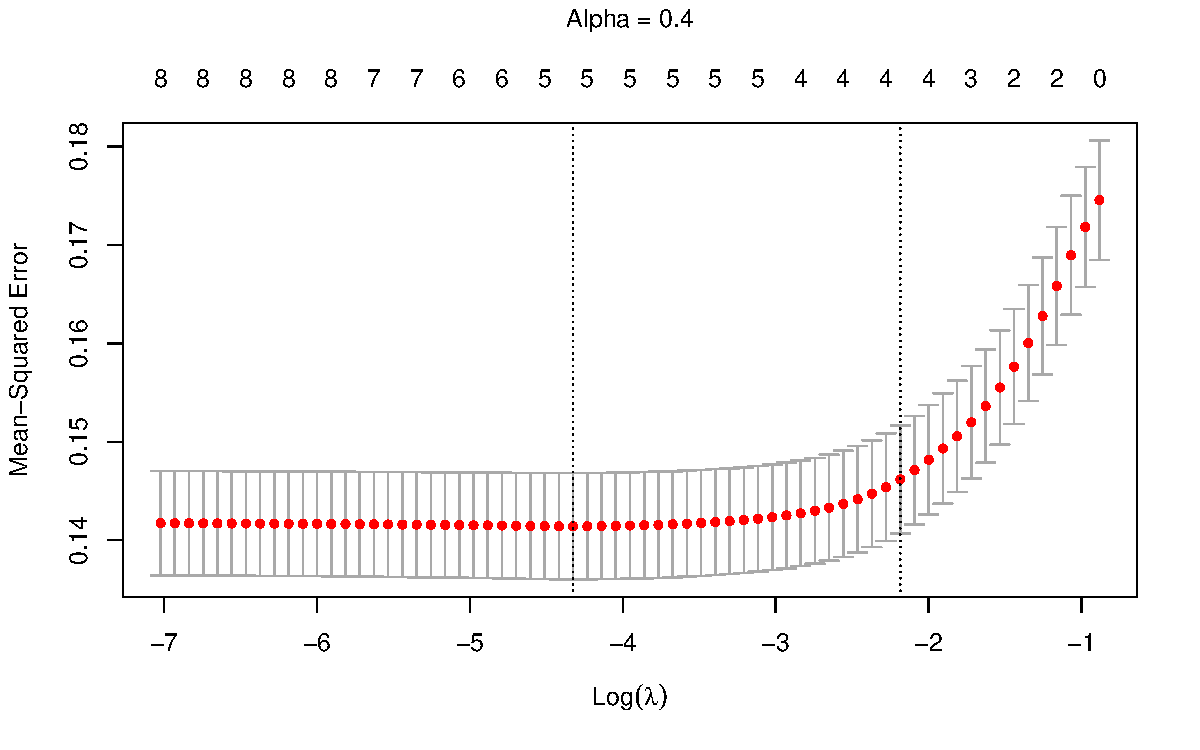
\includegraphics[width=\textwidth]{A2_files/figure-latex/unnamed-chunk-7-3}
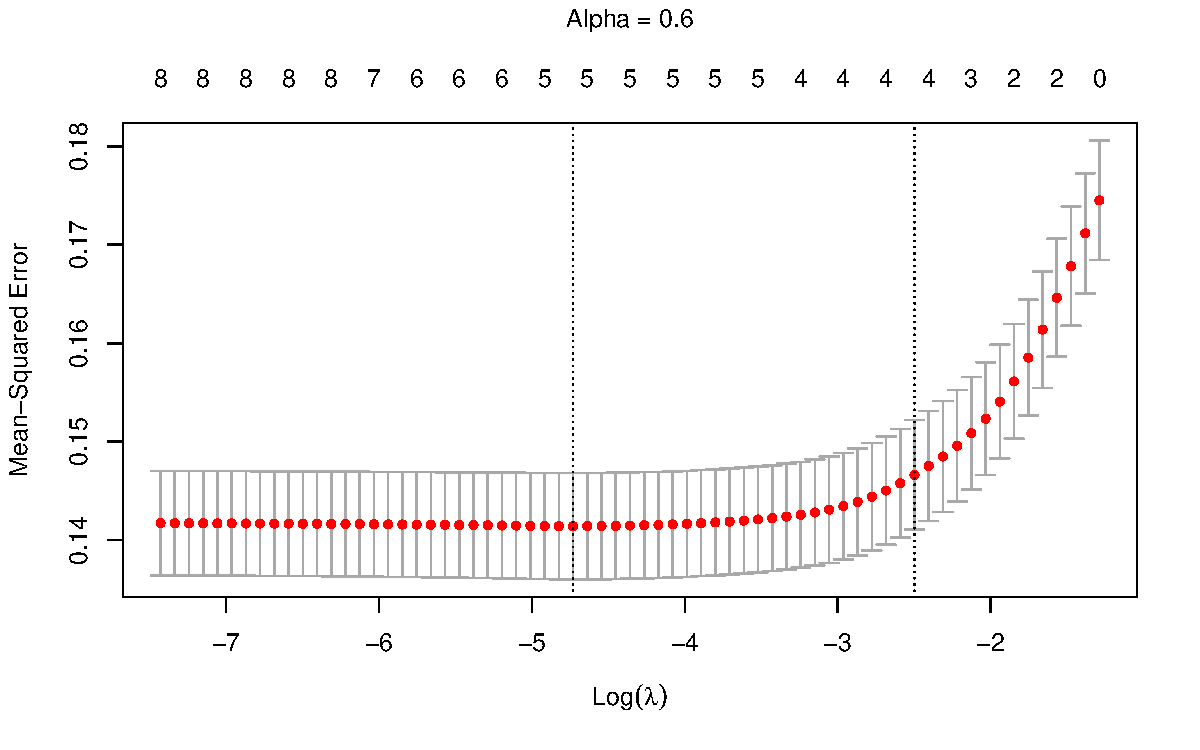
\includegraphics[width=\textwidth]{A2_files/figure-latex/unnamed-chunk-7-4}
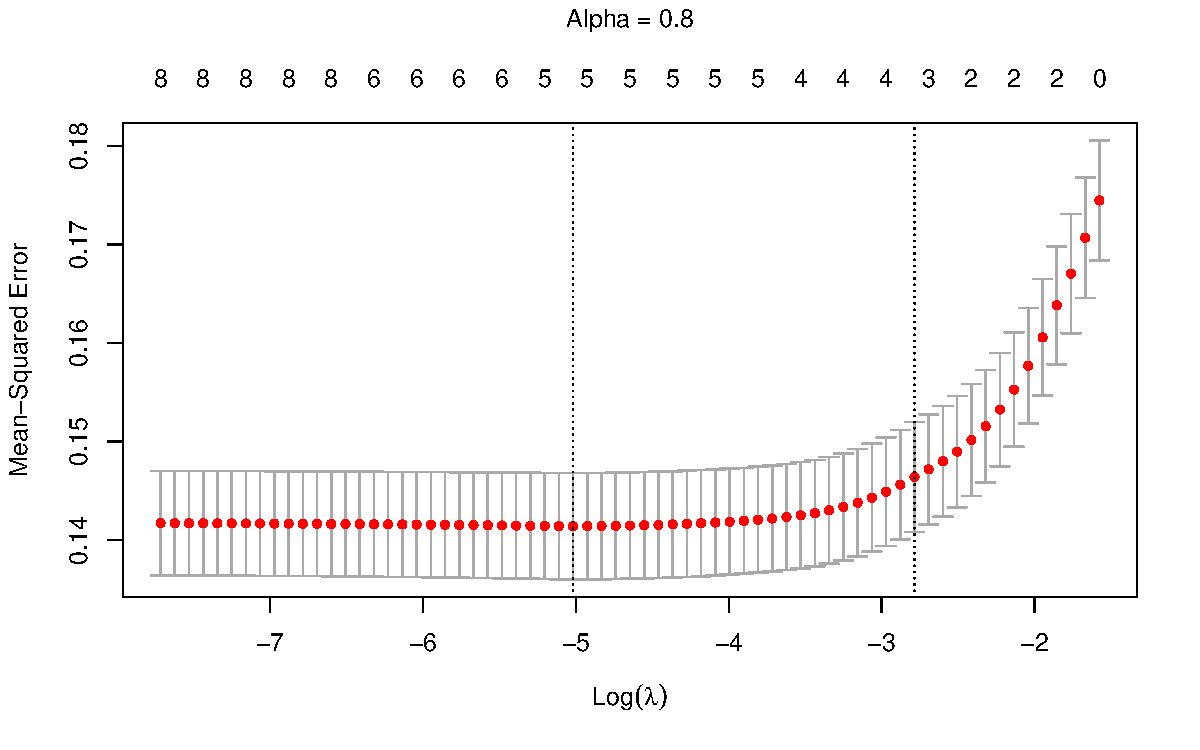
\includegraphics[width=\textwidth]{A2_files/figure-latex/unnamed-chunk-7-5}
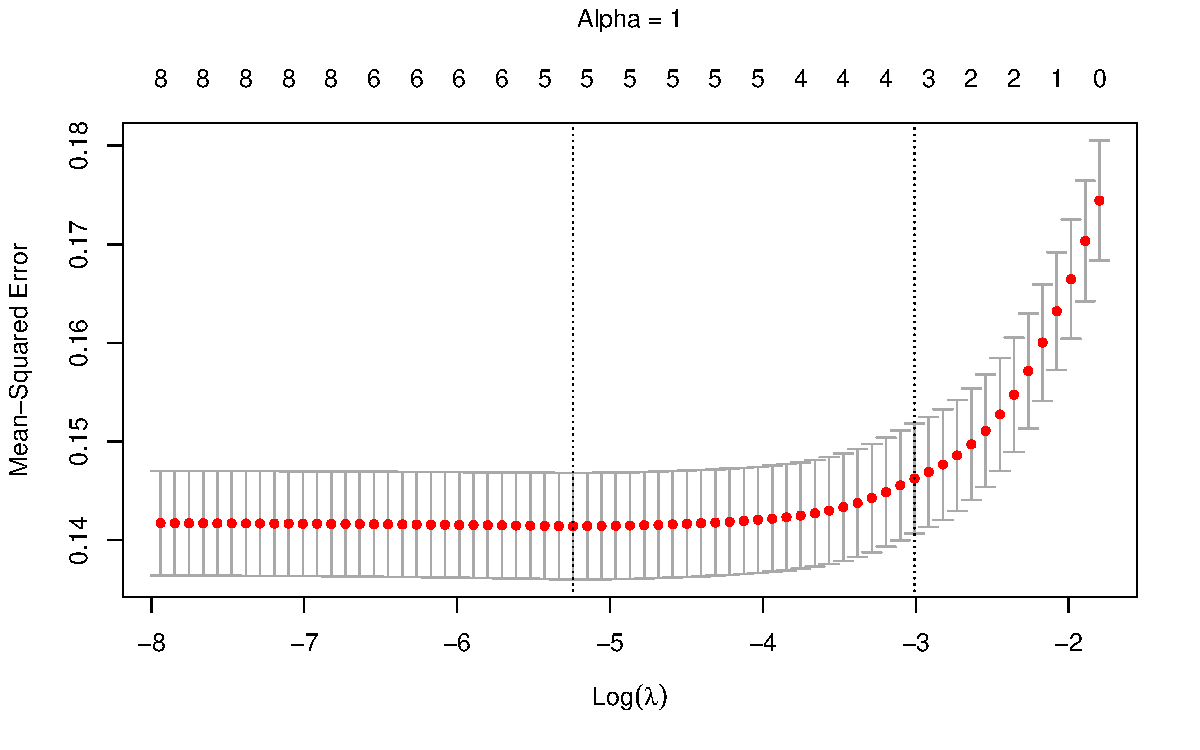
\includegraphics[width=\textwidth]{A2_files/figure-latex/unnamed-chunk-7-6}

This visualization helps in choosing an optimal lambda value , typically
via the 1-standard error rule or by selecting the lambda that minimizes
the cross-validation error.

Next, to select the best value for \(\lambda\), that balances model
simplicity and accuracy, for each fixed value of \(\alpha\) we look at
either the value that minimizes the cross-validation error (lambda.min)
or the 1-SE rule (lambda.1se), and then compare the selected models. We
extract these \(\lambda\) values from cv.glmnet and then fit the final
models on the full data set using these selected \(\lambda\) value. To
compare the selected models based on their complexity (number of
non-zero coefficients), predicted values, and MSE, we can use the coef
function to inspect the coefficients, make predictions with the predict
function, and then calculate MSE for each model. Table 2 summarizes all
that. The choice between lambda.min and lambda.1se involves a trade-off
between model simplicity and predictive accuracy. lambda.1se typically
leads to simpler models (with potentially slightly higher MSE). We
observe that as \(\alpha\) increases from 0.0 to 1.0, the number of
non-zero coefficients varies. The model with \(\alpha\) = 0.0 (ridge
regression) maintains 10 non-zero coefficients for both lambda.min and
lambda.1se. For other values of \(\alpha\) (moving towards lasso
regression), the number of non-zero coefficients tends to decrease,
indicating sparser models. This is especially visible for
\(\alpha = 1.0\) with only 5 or 6 non-zero coefficients, suggesting that
lasso regularization enforces the most sparsity. The least complex model
is the one with \(\alpha = 0.2\) using the lambda.1se criterion, having
only 5 non-zero coefficients, whereas the most complex models with
respect to the number of coefficients are all those with
\(\alpha = 0.0\). Regarding predicited values, the cv\_mse does not vary
significantly across different \(\alpha\) values, indicating that the
change in \(\alpha\) is not drastically affecting the model's predictive
ability in this case. The lowest cv\_mse for lambda.min appears at
\(\alpha = 1.0\) , suggesting that the lasso model at its optimal lambda
achieves a marginally better fit in terms of MSE. For the lambda.1se
criterion, the cv\_mse is slightly higher compared to the lambda.min,
which is expected as the 1-SE rule tends to select a simpler and more
generalizable model at the expense of a slight increase in error. In the
end, the choice between lambda.min and lambda.1se would depend on
whether the priority is on the lowest possible MSE or on model
simplicity.

\#\#Frage: classification performance - only if I have logistic
regression and binary outcome or?

\begin{longtable}[]{@{}rrlrr@{}}
\toprule()
alpha & lambda & criterion & non\_zero\_coefficients & cv\_mse \\
\midrule()
\endhead
0.0 & 0.0505227 & min & 10 & 0.1416001 \\
0.0 & 0.7502457 & 1se & 10 & 0.1468714 \\
0.2 & 0.0241132 & min & 7 & 0.1414149 \\
0.2 & 0.2049025 & 1se & 5 & 0.1467689 \\
0.4 & 0.0132321 & min & 6 & 0.1414132 \\
0.4 & 0.1124401 & 1se & 5 & 0.1461814 \\
0.6 & 0.0088214 & min & 6 & 0.1414171 \\
0.6 & 0.0822686 & 1se & 5 & 0.1466378 \\
0.8 & 0.0066160 & min & 6 & 0.1414202 \\
0.8 & 0.0617014 & 1se & 5 & 0.1464145 \\
1.0 & 0.0052928 & min & 6 & 0.1414225 \\
1.0 & 0.0493612 & 1se & 5 & 0.1462448 \\
\bottomrule()
\end{longtable}

Last, we inspect the best solution for \(\alpha = 1\) (lasso regression)
using the 1 − SE rule. This approach tends to prefer simpler models with
fewer non-zero coefficients, which can be advantageous for
interpretability and generalization. To see which variables were
selected (i.e., have non-zero coefficients) and their estimated
coefficients, we use the coef function from the glmnet package. We
observe here only 4 variables are selcted, and all have rather small
coefficients ans thus little influence on the response variable
`lwage76'. To assess the goodness-of-fit, we then calculate the
correlation between the predicted values from the model and the observed
values. Values closer to 1 or -1 indicating a stronger linear
relationship between predictions and actual outcomes. In this case the
correlation lies at 0.4293. This indicates a moderate postive linear
relationship between the predicted and observed values.The model has
some predictive power, but it is not capturing all of the variability in
the dependent variable.

\begin{verbatim}
## [1] "Non-zero coefficients (including intercept):"
\end{verbatim}

\begin{verbatim}
## 27 x 1 sparse Matrix of class "dgCMatrix"
##                       s1
## (Intercept) 5.542382e+00
## smsa66      .           
## smsa76      .           
## nearc2      .           
## nearc4      .           
## nearc4a     .           
## nearc4b     .           
## ed76        .           
## ed66        4.554928e-02
## age76       1.443958e-03
## daded       .           
## nodaded     .           
## momed       .           
## nomomed     .           
## momdad14    .           
## sinmom14    .           
## step14      .           
## south66     .           
## south76     .           
## famed       .           
## black       .           
## enroll76    .           
## kww         6.283247e-03
## iqscore     3.616473e-05
## mar76       .           
## libcrd14    .           
## exp76       .
\end{verbatim}

\begin{verbatim}
## [1] "Correlation between predicted and observed values for alpha = 1 (1-SE rule): 0.4293"
\end{verbatim}

\hypertarget{exercise-4}{%
\section{Exercise 4}\label{exercise-4}}

\hypertarget{exercise-5}{%
\section{Exercise 5}\label{exercise-5}}

\end{document}
